\let\negmedspace\undefined
\let\negthickspace\undefined
\documentclass[journal]{IEEEtran}
\usepackage[a5paper, margin=10mm, onecolumn]{geometry}
\usepackage{lmodern}
\usepackage{tfrupee}
\setlength{\headheight}{1cm}
\setlength{\headsep}{0mm}
\usepackage{gvv-book}
\usepackage{gvv}
\usepackage{cite}
\usepackage{amsmath,amssymb,amsfonts,amsthm}
\usepackage{algorithmic}
\usepackage{graphicx}
\usepackage{textcomp}
\usepackage{xcolor}
\usepackage{txfonts}
\usepackage{listings}
\usepackage{enumitem}
\usepackage{mathtools}
\usepackage{gensymb}
\usepackage{comment}
\usepackage[breaklinks=true]{hyperref}
\usepackage{tkz-euclide}
\usepackage{listings}
\usepackage{color}
\usepackage{array}
\usepackage{longtable}
\usepackage{calc}
\usepackage{multirow}
\usepackage{hhline}
\usepackage{ifthen}
\usepackage{lscape}
\usepackage{multicol}


% Footer macro
\newcommand{\qfooter}{%
  \begin{flushright}\footnotesize\textbf{[GATE EE 2025]}\end{flushright}\vspace{1em}%
}

\begin{document}
\bibliographystyle{IEEEtran}
\vspace{3cm}
\title{BM22 -BIOMEDICAL}
\author{EE25BTECH11009 - ANSHU KUMAR RAM}
{\let\newpage\relax\maketitle}

\begin{enumerate}

% Q1
\item The \underline{\hspace{2cm}} is too high for it to be considered \underline{\hspace{2cm}}.
\begin{enumerate}
\begin{multicols}{4}
\item fair / fare
\item faer / fair
\item fare / fare
\item fare / fair
\end{multicols}
\qfooter
\end{enumerate}

% Q2
\item A function $y(x)$ is defined in the interval $[0, 1]$ on the $x$-axis as
\begin{align}
y(x) = 
\begin{cases}
2 & 0 \leq x < \frac{1}{3} \\
3 & \frac{1}{3} \leq x < \frac{3}{4} \\
1 & \frac{3}{4} \leq x \leq 1
\end{cases}
\end{align}
Which one of the following is the area under the curve for the interval $[0, 1]$ on the $x$-axis?
\begin{enumerate}
\begin{multicols}{4}
\item $\frac{5}{6}$
\item $\frac{6}{5}$
\item $\frac{13}{6}$
\item $\frac{6}{13}$
\end{multicols}
\qfooter
\end{enumerate}

% Q3
\item Let $r$ be a root of the equation $x^2 + 2x + 6 = 0$. Then the value of the expression $(r+2)(r+3)(r+4)(r+5)$ is
\begin{enumerate}
\begin{multicols}{4}
\item 51
\item $-51$
\item 126
\item $-126$
\end{multicols}
\qfooter
\end{enumerate}

% Q4
\item Given below are four statements.\\
Statement 1: All students are inquisitive.\\
Statement 2: Some students are inquisitive.\\
Statement 3: No student is inquisitive.\\
Statement 4: Some students are not inquisitive.\\
From the given four statements, find the two statements that CANNOT BE TRUE simultaneously, assuming that there is at least one student in the class.
\begin{enumerate}
\begin{multicols}{2}
\item Statement 1 and Statement 3
\item Statement 1 and Statement 2
\item Statement 2 and Statement 4
\item Statement 3 and Statement 4
\end{multicols}
\qfooter
\end{enumerate}

% Q5
\item A palindrome is a word that reads the same forwards and backwards. In a game 
of words, a player has the following two plates painted with letters.

\begin{figure}[h]
\centering
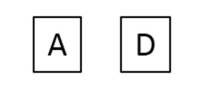
\includegraphics[width=0.38\columnwidth]{figs/q5.png}
% Adjust width as needed
\end{figure}

From the additional plates given in the options below, which one of the combinations 
of additional plates would allow the player to construct a five-letter palindrome? 
The player should use all the five plates exactly once. The plates can be rotated 
in their plane.

\begin{enumerate}
\item 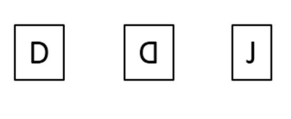
\includegraphics[width=0.17\columnwidth]{figs/q5a.png}
\item 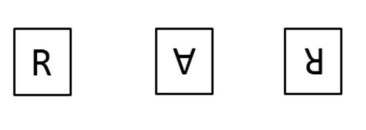
\includegraphics[width=0.17\columnwidth]{figs/q5b.png}
\item 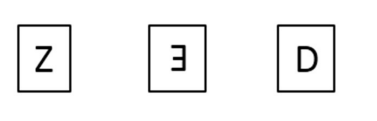
\includegraphics[width=0.17\columnwidth]{figs/q5c.png}
\item 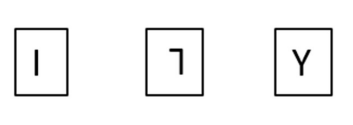
\includegraphics[width=0.17\columnwidth]{figs/q5d.png}
\qfooter
\end{enumerate}


% Q6
\item Some people believe that ``what gets measured, improves.'' Some others believe that ``what gets measured, gets gamed.'' One possible reason for the difference in the beliefs is the work culture in organizations. In organizations with good work culture, metrics help improve outcomes. However, the same metrics are counterproductive in organizations with poor work culture.\\
Which one of the following is the CORRECT logical inference based on the information in the above passage?
\begin{enumerate}
\item Metrics are useful in organizations with poor work culture
\item Metrics are useful in organizations with good work culture
\item Metrics are always counterproductive in organizations with good work culture
\item Metrics are never useful in organizations with good work culture
\qfooter
\end{enumerate}

% Q7
\item In a recently conducted national entrance test, boys constituted $65\%$ of those who appeared for the test. Girls constituted the remaining candidates and they accounted for $60\%$ of the qualified candidates.\\
Which one of the following is the correct logical inference based on the information provided in the above passage?
\begin{enumerate}
\item Equal number of boys and girls qualified
\item Equal number of boys and girls appeared for the test
\item The number of boys who appeared for the test is less than the number of girls who appeared
\item The number of boys who qualified the test is less than the number of girls who qualified
\qfooter
\end{enumerate}

% Q8
\item A box contains five balls of same size and shape. Three of them are green coloured balls and two of them are orange coloured balls. Balls are drawn from the box one at a time. If a green ball is drawn, it is not replaced. If an orange ball is drawn, it is replaced with another orange ball.\\
First ball is drawn. What is the probability of getting an orange ball in the next draw?
\begin{enumerate}
\begin{multicols}{4}
\item $\frac{1}{2}$
\item $\frac{8}{25}$
\item $\frac{19}{50}$
\item $\frac{23}{50}$
\end{multicols}
\qfooter
\end{enumerate}

% Q9
\item The corners and mid-points of the sides of a triangle are named using the distinct letters P, Q, R, S, T and U, but not necessarily in the same order.\\
Consider the following statements:
\begin{itemize}
    \item The line joining P and R is parallel to the line joining Q and S.
    \item P is placed on the side opposite to the corner T.
    \item S and U cannot be placed on the same side.
\end{itemize}
Which one of the following statements is correct based on the above information?
\begin{enumerate}
\item P cannot be placed at a corner
\item S cannot be placed at a corner
\item U cannot be placed at a mid-point
\item R cannot be placed at a corner
\qfooter
\end{enumerate}

% Q10
\item A plot of land must be divided between four families. They want their individual plots to be similar in shape, not necessarily equal in area. The land has equally spaced poles, marked as dots in the below figure. Two ropes, R1 and R2, are already present and cannot be moved.

\begin{figure}[h]
\centering
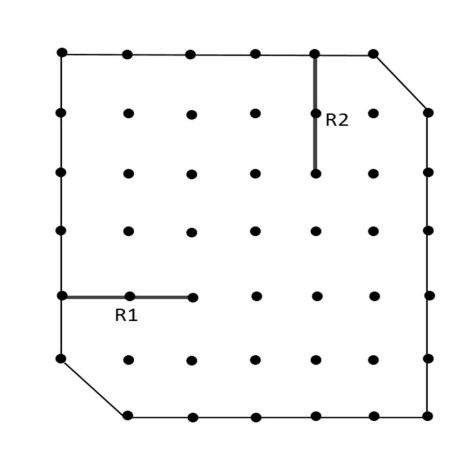
\includegraphics[width=0.5\columnwidth]{figs/q10.png}
\end{figure}
\newpage
What is the least number of additional straight ropes needed to create the desired plots? A single rope can pass through three poles that are aligned in a straight line.
\begin{enumerate}
\begin{multicols}{4}
\item 2
\item 4
\item 5
\item 3
\end{multicols}
\qfooter
\end{enumerate}


% Q11
\item If the given matrices
\begin{align}
A = \begin{bmatrix} 2 & -4 \\ 2 & 3 \end{bmatrix}, \quad
I = \begin{bmatrix} 1 & 0 \\ 0 & 1 \end{bmatrix},
\end{align}
satisfy the equation
\begin{align}
I - kA = A^2,
\end{align}
the value of coefficient \(k\) is\underline{\hspace{2cm}}.

\begin{enumerate}
\begin{multicols}{4}
\item 1
\item 2
\item 0
\item 4
\end{multicols}
\end{enumerate}
\qfooter

% Q12
\item Evaluation of the integral
\begin{align}
\int \frac{dx}{2 - x^2}
\end{align}
results in

\begin{enumerate}
\begin{multicols}{4}
\item \(c + \frac{1}{\sqrt{2}} \sin^{-1} \frac{x}{\sqrt{2}}\)
\item \(c + \frac{1}{\sqrt{2}} \cos^{-1} \frac{x}{\sqrt{2}}\)
\item \(c + \sin^{-1} \frac{x}{\sqrt{2}}\)
\item \(c + \cos^{-1} \frac{x}{\sqrt{2}}\)
\end{multicols}
\end{enumerate}
\qfooter

% Q13
\item If 
\begin{align}
\vec{V} = a \hat{i} + b \hat{j} + c \hat{k},
\end{align}
identify the INVALID operation on \(\vec{V}\).

\begin{enumerate}
\begin{multicols}{4}
\item \((\vec{V} \times \nabla) \cdot \nabla\)
\item \((\vec{V} \cdot \nabla) \times \nabla\)
\item \((\vec{V} \cdot \nabla) \nabla\)
\item \(\vec{V} \nabla \times \nabla\)
\end{multicols}
\end{enumerate}
\qfooter

% Q14
\item \(x(t)\) is a real continuous-time signal whose magnitude frequency response \(|X(j \omega)|\) is shown below. After sampling \(x(t)\) at 100 rad/s, the spectral point \(P\) is down-converted to\underline{\hspace{2cm}} rad/s in the spectrum of the sampled signal.

\begin{figure}[H]
\centering
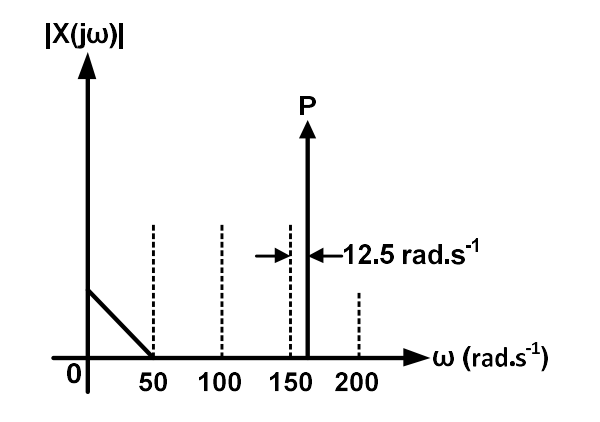
\includegraphics[width=0.6\columnwidth]{figs/q14.png}
% Placeholder for frequency response figure
\end{figure}

\begin{enumerate}
\begin{multicols}{4}
\item 12.5
\item 25
\item 6.25
\item 37.5
\end{multicols}
\end{enumerate}
\qfooter

% Q15
\item Discrete signals $x[n]$ and $y[n]$ are shown below. The cross-correlation $r_{xy}$ is \underline{\hspace{2cm}}.
\begin{figure}[H]
\centering
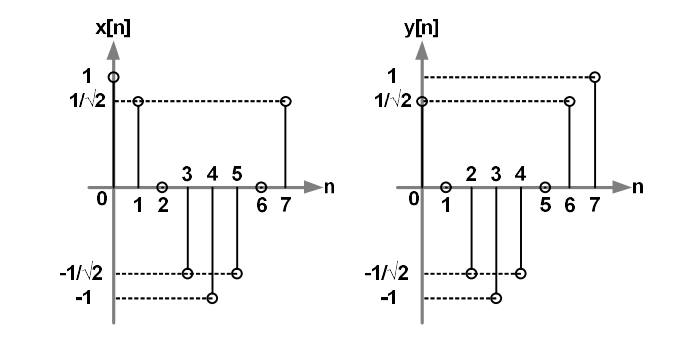
\includegraphics[width=0.5\columnwidth]{figs/q15.png}
% Placeholder for discrete signals image
\end{figure}

\begin{enumerate}
\begin{multicols}{4}
\item $2\sqrt{2}$
\item $\frac{1}{2}\sqrt{2}$
\item $\frac{1}{2}$
\item $\frac{1}{\sqrt{2}}$
\end{multicols}
\end{enumerate}


% Q16
\item In the circuit diagram shown below, the logic gates operate with a supply voltage of 1 V. NAND and XNOR have 200 ps and 400 ps input-to-output delay, respectively.  
At time \(t = T\), \(A(t) = 0\), \(B(t) = 1\), and \(Z(t) = 0\). When the inputs are changed to \(A(t) = 1\), \(B(t) = 0\) at \(t = 2T\), a 1 V pulse is observed at \(Z\). The pulse width of the 1 V pulse is \underline{\hspace{2cm}} ps.

\begin{figure}[H]
\centering
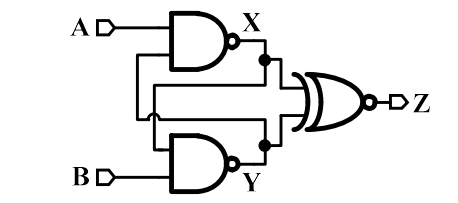
\includegraphics[width=0.5\columnwidth]{figs/q16.png}
% Placeholder for circuit diagram
\end{figure}

\begin{enumerate}
\begin{multicols}{4}
\item 100
\item 200
\item 400
\item 600
\end{multicols}
\end{enumerate}
\qfooter

% Q17
\item Input bits \(X\) and \(Y\) are added using the combinational logic shown below. \(S\) represents the sum of the two bits. For a correct implementation of the sum, the signals \(D_0, D_1, D_2, D_3\) are\underline{\hspace{2cm}}, respectively.

\begin{figure}[H]
\centering
 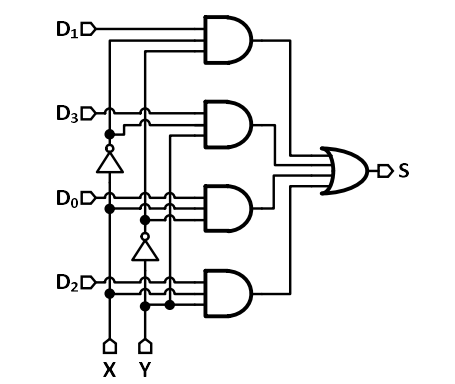
\includegraphics[width=0.5\columnwidth]{figs/q17.png}
 % Placeholder for combinational logic figure
\end{figure}

\begin{enumerate}
\begin{multicols}{4}
\item 1, 0, 0, 1
\item 0, 1, 0, 1
\item 1, 0, 1, 1
\item 0, 1, 1, 0
\end{multicols}
\end{enumerate}
\qfooter

% Q18
\item The time delay between the peaks of the voltage signals \(v_1(t) = 2\cos(6t + 60^\circ)\) and \(v_2(t) = -3 \sin(6t)\) is\underline{\hspace{2cm}} s.

\begin{enumerate}
\begin{multicols}{4}
\item \(\frac{300\pi}{360}\)
\item \(\frac{10\pi}{360}\)
\item \(\frac{50\pi}{360}\)
\item \(\frac{200\pi}{360}\)
\end{multicols}
\end{enumerate}
\qfooter

% Q19
\item For the balanced Owen-bridge circuit shown in the figure, the values of \(L_1\) and \(R_1\) are:

\begin{figure}[H]
\centering
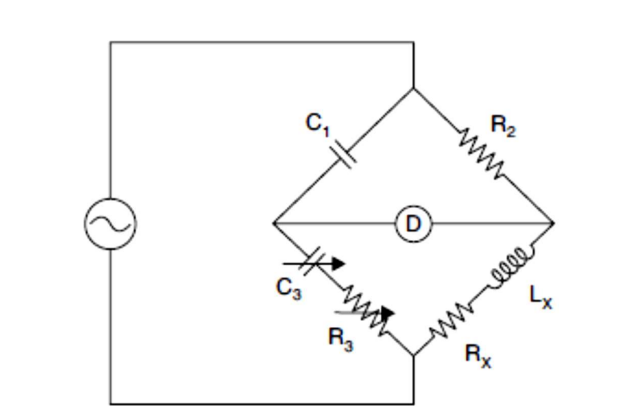
\includegraphics[width=0.4\columnwidth]{figs/q19.png}
% Placeholder for Owen-bridge circuit diagram
\end{figure}

\begin{enumerate}
\item \(L_1 = R_1 R_2 C_1,\quad R_1 = \frac{R_4 C_1}{C_2}\)
\item \(L_1 = R_2 R_3 C_1,\quad R_1 = \frac{R_4 C_2}{C_1}\)
\item \(L_1 = R_3 R_4 C_1,\quad R_1 = \frac{R_2 C_1}{C_2}\)
\item \(L_1 = R_1 R_2 C_1,\quad R_1 = \frac{R_3 C_2}{C_1}\)

\end{enumerate}
\qfooter

% Q20
\item Myopia occurs when the focal point falls \underline{\hspace{2cm}}the retina. This can be corrected using a \underline{\hspace{2cm}} lens.

\begin{enumerate}
\begin{multicols}{2}
\item in front of, convex
\item behind, convex
\item in front of, concave
\item behind, concave
\end{multicols}
\end{enumerate}
\qfooter


% Q21
\item Choose the correct sequence for the direction of blood flow in a healthy human being starting and ending with the left ventricle.

\begin{enumerate}

\item Left ventricle → Aorta → Systemic arteries → Systemic veins → Vena cavae → Pulmonary vein → Pulmonary artery → Right ventricle → Left ventricle
\item Left ventricle → Aorta → Systemic arteries → Systemic veins → Vena cavae → Right ventricle → Pulmonary artery → Pulmonary vein → Left ventricle
\item Left ventricle → Systemic arteries → Aorta → Systemic veins → Right ventricle → Pulmonary artery → Pulmonary vein → Left ventricle
\item Left ventricle → Aorta → Systemic arteries → Vena cavae → Systemic veins → Right ventricle → Pulmonary artery → Pulmonary vein → Left ventricle

\end{enumerate}
\qfooter

% Q22
\item In a healthy adult, which one of the following regions of the brain contains primarily white matter?

\begin{enumerate}
\begin{multicols}{2}
\item Cerebral cortex
\item Basal ganglia
\item Limbic system
\item Corpus callosum
\end{multicols}
\end{enumerate}
\qfooter

% Q23
\item Skeletal muscles are recruited to lift loads. If the force generated in the muscle due to contraction is not sufficient to lift the load, it is known as \underline{\hspace{2cm}} contraction.

\begin{enumerate}
\begin{multicols}{4}
\item Isometric
\item Isotonic
\item Isokinetic
\item Isoinertial
\end{multicols}
\end{enumerate}
\qfooter

% Q24
\item Backscattered electron detector of a scanning electron microscope is used to

\begin{enumerate}
\item study surface topography of the sample
\item quantify surface roughness
\item measure atomic number
\item contrast areas with different chemical compositions
\end{enumerate}
\qfooter

% Q25
\item In the process of obtaining a Magnetic Resonance Image (MRI), the terms T1 and T2 time constants of the material are very crucial to decide on getting suitable weighted images. Choose the correct explanation relating to these two constants from the following options.

\begin{enumerate}
\item T1 is the spin-lattice or longitudinal relaxation time, and T2 is the spin-spin or transverse relaxation time
\item T1 and T2 indicate the durations that Free Induction Decay (FID) signal to be recorded in x and y axes directions, respectively
\item T1 and T2 refer to the durations of flipping pulses used to tilt the resultant magnetic vector into x-y plane and inverse z-direction, respectively
\item T1 is the spin-spin or transverse relaxation time, and T2 is the spin-lattice or longitudinal relaxation time
\end{enumerate}
\qfooter

% Q26
\item Given \(x\) is real, identify all the even-functions among the following:

\begin{enumerate}
\begin{multicols}{4}
\item \(x/x\)
\item \(x \cos x\)
\item \(\sin^2 x\)
\item \(e^{-x}\)
\end{multicols}
\end{enumerate}
\qfooter

% Q27
\item An ideal coronary stent should

\begin{enumerate}

\item be thromboresistant
\item promote accumulation of smooth muscle cells
\item be fatigue resistant
\item support deposition of extracellular matrix

\end{enumerate}
\qfooter

% Q28
\item Which of the following statements related to the safety of biomedical instruments are TRUE?

\begin{enumerate}
\item When a person is exposed to an electrical hazard, let-go current is defined as the maximum current at which the subject can withdraw voluntarily
\item Microshock is a physiological response resulting from an electrical current passing through heart
\item The patient in an intensive care unit is being exposed to the danger of microshock because of using internal conductive electrodes in the vicinity of the heart
\item The 50 Hz safe current limit for a microshock is greater than 50 mA
\end{enumerate}
\qfooter

% Q29
\item Which of the following statements related to the operating principle of pulse oximetry are CORRECT?

\begin{enumerate}
\item Pulse oximeter can non-invasively determine arterial oxygen saturation (SpO2) by analyzing the light transmitted through the skin during the systolic phase of the blood flow through the tissue
\item In a pulse oximeter, isosbestic wavelength is the wavelength at which Hb and HbO2 have same optical absorbance
\item Pulse oximeter can accurately determine the SpO2 of blood by computing the ratio of absorbances at 660 nm and 905 nm wavelengths
\item Pulse oximeter can accurately determine the SpO2 of blood by computing the ratio of absorbances at 850 nm and 950 nm wavelengths
\end{enumerate}
\qfooter

% Q30
\item Which of the following statements related to biomedical measurements are TRUE?

\begin{enumerate}
\item Electrical activity of neurons in the peripheral nervous system can be measured by ENG
\item Electrical activity of the retina in response to light stimulus can be measured using EOG
\item In a human EEG, Gamma waves are high frequency waves compared to Beta, Delta, and Theta waves
\item P wave in ECG manifests ventricular repolarization
\end{enumerate}
\qfooter

% Q31
\item Which of the following mechanical prosthetic valves were invented as a replacement for diseased heart valves?

\begin{enumerate}
\begin{multicols}{2}
\item Globe valve
\item Ball and cage valve
\item Bi-leaflet valve
\item Swing check valve
\end{multicols}
\end{enumerate}
\qfooter

% Q32
\item Due to the current COVID pandemic conditions, assume that positive or negative status of any individual are equally likely. There are 3 members in a family. If one of the members has tested COVID positive, the conditional probability that at least 2 members are COVID positive is \underline{\hspace{2cm}}(rounded off to three decimal places).

\qfooter

% Q33
\item A series RLC circuit with \(R = 10\ \Omega\), \(L = 50\ \text{mH}\) and \(C = 100\ \mu \text{F}\) connected to 200 V, 50 Hz supply consumes power \(P\). The value of \(L\) is changed such that this circuit consumes same power \(P\) but operates with lagging power factor. The new value of \(L\) is \underline{\hspace{2cm}} mH (rounded off to two decimal places).

\qfooter

% Q34
\item The thickness of piezoelectric crystal (PZT5A) used in ultrasound applications will determine the resonant frequency of the transducer. To work at a resonance frequency of 5 MHz, the thickness of a PZT5A transducer must be \underline{\hspace{2cm}}mm (rounded off to three decimal places).

Given: The velocity of sound in PZT5A is 4350 m.s\(^{-1}\).

\qfooter

% Q35
\item Power consumed by the $3\,\Omega$ resistor is $12\,\mathrm{W}$ in the given circuit. The value of the resistor $R$ in the circuit is \rule{2cm}{0.15mm}\,$\Omega$.

\begin{figure}[h]
\centering
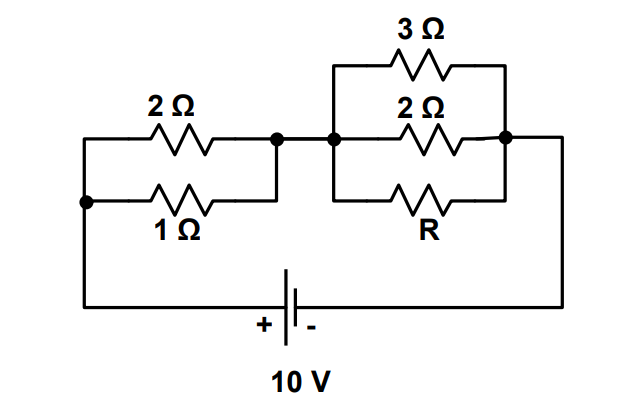
\includegraphics[width=0.38\columnwidth]{figs/q35.png}
\end{figure}

\qfooter


% Q36
\item In the complex \(z\)-domain, the value of the integral
\begin{align}
\oint_C \frac{i}{z^3 - 9z + 3} dz
\end{align}
is

\begin{enumerate}
\begin{multicols}{4}
\item \(\pi i \frac{6}{81}\)
\item \(\pi i \frac{6}{81}\) (different sign)
\item \(\pi i \frac{6}{81}\) (another sign form)
\item \(\pi i \frac{6}{81}\) (yet another sign form)
\end{multicols}
\end{enumerate}
\qfooter

% Q37
\item Solution of the differential equation
\begin{align}
x \frac{dy}{dx} = \cos y
\end{align}
is

\begin{enumerate}
\begin{multicols}{2}
\item \(y = c e^x - 2 \cos x \sin x\)
\item \(y = c e^x + 2 \cos x \sin x\)
\item \(y = c e^{-x} + 2 \cos x \sin x\)
\item \(y = c e^{-x} - 2 \cos x \sin x\)
\end{multicols}
\end{enumerate}
\qfooter

% Q38
\item An input $x(t)$ is applied to a system with a frequency transfer function given by $H(j\omega)$ as shown below. The magnitude and phase response of the transfer function are shown below. If $y(t_1) = 0$ for $x(t) = u(t)$, the time $t_1\ (>0)$ is \rule{2cm}{0.15mm}\,$\mu$s.

\begin{figure}[h]
\centering
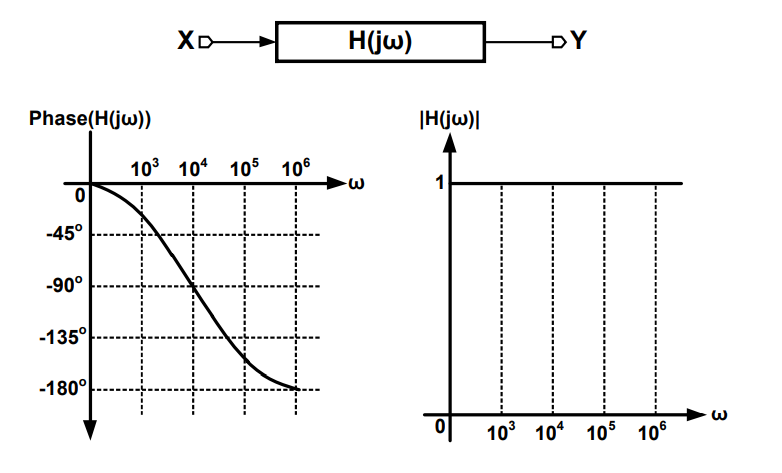
\includegraphics[width=0.5\columnwidth]{figs/q38.png}
% Adjust width/file name as required
\end{figure}

\begin{enumerate}
\begin{multicols}{2}
\item $100\ln(2)$\\
\item $10\ln(2)$\\
\item $1000\ln(2)$\\
\item $\ln(2)$\\
\end{multicols}
\qfooter
\end{enumerate}


% Q39
\item The block diagram of a two-tap high-pass FIR filter is shown below. The filter transfer function is given by $H(z) = Y(z)/X(z)$.  
If ratio of the maximum to minimum value of $H(z)$ is $2$ and $|H(z)|_{max}= 1$, the coefficients $\beta_1$ and $\beta_2$ are \rule{1.2cm}{0.15mm} and \rule{1.2cm}{0.15mm}, respectively.

\begin{figure}[h]
\centering
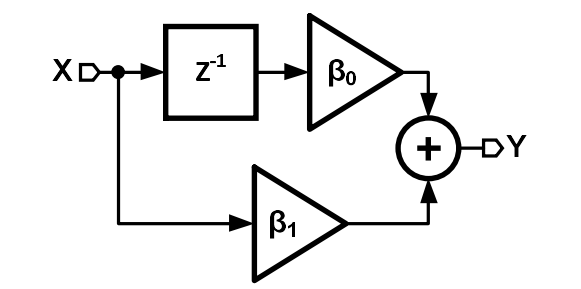
\includegraphics[width=0.48\columnwidth]{figs/q39.png}
% Adjust width/filename as required
\end{figure}

\begin{enumerate}
\begin{multicols}{2}
\item $0.75,\ -0.25$
\item $0.67,\ 0.33$
\item $0.60,\ -0.40$
\item $-0.64,\ 0.36$
\end{multicols}
\qfooter
\end{enumerate}

% Q40
\item The block diagrams of an ideal system and a real system with their impulse responses are shown below. An auxiliary path is added to the delayed impulse response in the real system.   
For a unit impulse input $(x(t) = \delta(t))$ to both systems, gain $\beta$ is chosen such that $y(4T)$ is same for both systems. The value of $\beta$ is \rule{2cm}{0.15mm}.

\begin{figure}[h]
\centering
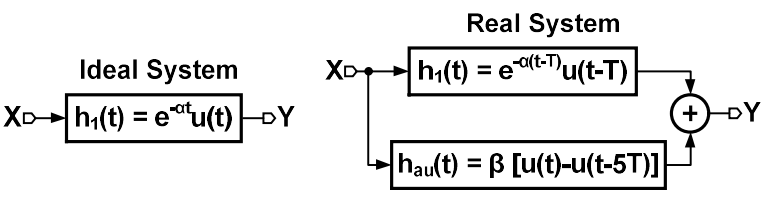
\includegraphics[width=0.48\columnwidth]{figs/q40.png}
% Adjust width/filename as required
\end{figure}

\begin{enumerate}
\begin{multicols}{2}
\item $e^{-4}(1 - e^{-4})$\\
\item $-e^{-4}(1 - e^{-4})$\\
\item $-e^{-4}(1 - e^{-1})$\\
\item $e^{-1}(1 - e^{-4})$\\
\end{multicols}
\qfooter
\end{enumerate}

% Q41
\item A filter is designed using opamps, resistors, and capacitors as shown below. Opamps are ideal with infinite gain and infinite bandwidth. If $V_o(s)/V_i(s)$ is an all-pass transfer function, the value of resistor $R_2$ is \rule{2cm}{0.15mm}\ k$\Omega$.

\begin{figure}[h]
\centering
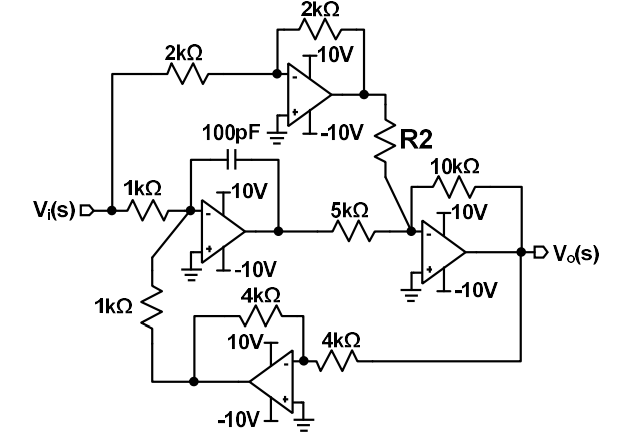
\includegraphics[width=0.48\columnwidth]{figs/q41.png}
% Adjust width/filename as required
\end{figure}

\begin{enumerate}
\begin{multicols}{4}
\item $1$\
\item $10$\
\item $5$\
\item $2$\
\end{multicols}
\qfooter
\end{enumerate}

% Q42
\item If \( g(t) = \frac{df(t)}{dt} \), and \( F(s) = \frac{1 + s}{s^2 + 12s + 32} \) where \( F(s) \) is the Laplace transform of the function \( f(t) \), then the value of \( g(t) \) at \( t=0 \) is \underline{\hspace{2cm}}.

\begin{enumerate}
\begin{multicols}{4}
\item -11
\item -5
\item -17
\item \(\infty\)
\end{multicols}
\end{enumerate}
\qfooter

% Q43
\item Consider the Einthoven’s triangle of frontal ECG for the 3 electrodes RA, LA and LL shown in the figure. The augmented lead vectors bisect the bipolar lead vectors. At the peak of R wave, the cardiac vector $M$ points vertically downwards with $|M| = 5\ \text{mV}$.  
The voltages on leads I and II are \rule{1.5cm}{0.15mm} mV and \rule{1.5cm}{0.15mm} mV, respectively.

\begin{figure}[h]
\centering
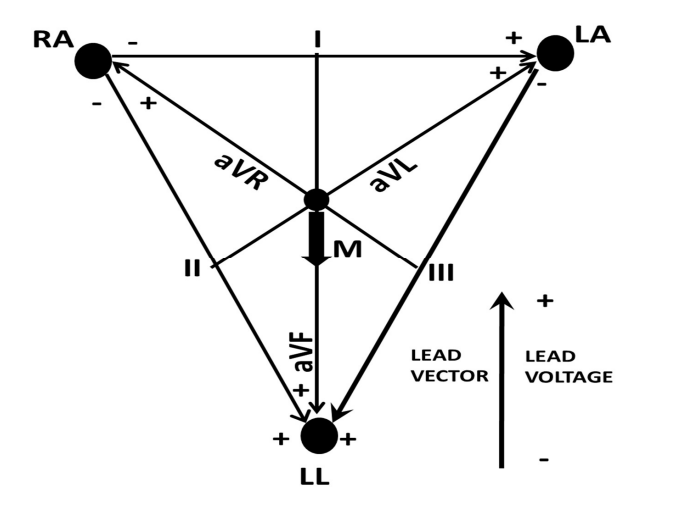
\includegraphics[width=0.45\columnwidth]{figs/q43.png}
% Substitute with actual image file
\end{figure}

\begin{enumerate}
\begin{multicols}{4}
\item $0,\ 4.33$
\item $2.17,\ 0$
\item $0,\ 2.17$
\item $4.33,\ 0$
\end{multicols}
\qfooter
\end{enumerate}


% Q44
\item Which one of the following statements is TRUE?

\begin{enumerate}
\begin{multicols}{4}
\item A myelinated axon has a greater ATP requirement than an unmyelinated axon of the same diameter and length
\item An unmyelinated axon has a greater ATP requirement than a myelinated axon of the same diameter and length
\item An unmyelinated axon has the same ATP requirement as a myelinated axon of the same diameter and length
\item An unmyelinated axon always has a greater ATP requirement than a myelinated axon irrespective of their diameter and length
\end{multicols}
\end{enumerate}
\qfooter

% Q45
\item The deltoid muscle connects the humerus to the shoulder blade and facilitates outstretching of the arm as shown in the figure. The humerus is connected to the shoulder blade with a ball and socket joint.  
Assume the equivalent weight ($W$) of the arm to be $30\ \text{N}$ and acts vertically down at a horizontal distance of $30\ \text{cm}$.  
Assume that the deltoid muscle is connected to the humerus at a distance of $15\ \text{cm}$ and makes an average angle of $20^\circ$ with the horizontal. The magnitude of tension in the deltoid muscle is \underline{\hspace{2cm}} N.

\begin{figure}[h]
\centering
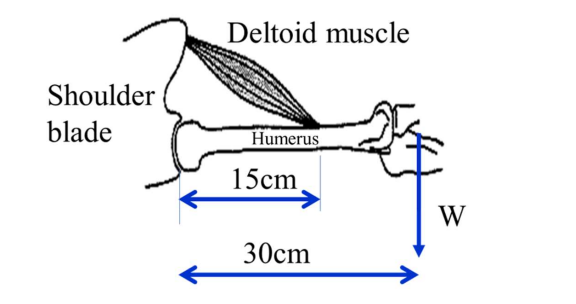
\includegraphics[width=0.45\columnwidth]{figs/q45.png}
% Substitute with actual image file
\end{figure}

\begin{enumerate}
\begin{multicols}{4}
\item 31.9
\item 63.8
\item 87.7
\item 175.4
\end{multicols}
\qfooter
\end{enumerate}


% Q46
\item For blood flow through arteries, which one of the following relations approximates the pulse wave propagation speed \( C \) as a function of the inner diameter \( D \) of the artery, wall thickness \( t \), modulus of elasticity \( E \), and fluid density \( \rho \)?

\begin{enumerate}
\begin{multicols}{4}
\item \(\displaystyle C = \frac{D}{t} \sqrt{\frac{E}{\rho}}\)
\item \(\displaystyle C = \frac{t}{D} \sqrt{\frac{E}{\rho}}\)
\item \(\displaystyle C = \sqrt[3]{\frac{E}{\rho}} \frac{t}{D}\)
\item \(\displaystyle C = \frac{t}{D} \frac{E}{\rho}\)
\end{multicols}
\end{enumerate}
\qfooter

% Q47
\item A person has a total blood volume of 5 L. Out of this total, assume that 4 L is contained in the systemic circulation and 1 L in pulmonary circulation. The cardiac output of the person is 5 L.min\(^{-1}\). Time taken for a drop of blood to go from right ventricle to left ventricle is \underline{\hspace{2cm}} s.

\begin{enumerate}
\begin{multicols}{4}
\item 60
\item 20
\item 15
\item 12
\end{multicols}
\end{enumerate}
\qfooter

% Q45
\item The deltoid muscle connects the humerus to the shoulder blade and facilitates outstretching of the arm as shown in the figure. The humerus is connected to the shoulder blade with a ball and socket joint.  
Assume the equivalent weight ($W$) of the arm to be $30\ \text{N}$ and acts vertically down at a horizontal distance of $30\ \text{cm}$.  
Assume that the deltoid muscle is connected to the humerus at a distance of $15\ \text{cm}$ and makes an average angle of $20^\circ$ with the horizontal. The magnitude of tension in the deltoid muscle is N.

\begin{figure}[h]
\centering
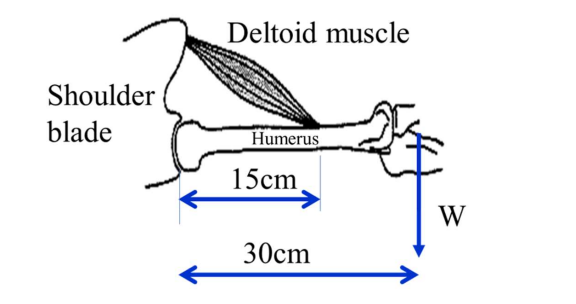
\includegraphics[width=0.45\columnwidth]{figs/q45.png}
% Substitute with actual image file
\end{figure}

\begin{enumerate}
\begin{multicols}{4}
\item 31.9
\item 63.8
\item 87.7
\item 175.4
\end{multicols}
\qfooter
\end{enumerate}

% Q49
\item Consider two radionuclides P and Q. Suppose the half-life of P (\( t_{1/2}^P \)) is four times that of Q (\( t_{1/2}^Q \)). At time \( t = 0 \), there are \( N_0 \) atoms of both radionuclides. When will the radioactivity of the two radionuclides be equal?

\begin{enumerate}
\begin{multicols}{4}
\item \( t = t_{1/2}^P \)
\item \( t = 0.66 t_{1/2}^P \)
\item \( t = 0.75 t_{1/2}^P \)
\item \( t = 1.5 t_{1/2}^P \)
\end{multicols}
\end{enumerate}
\qfooter

% Q50
\item In a biological study, the experimental values measured from 6 subjects are given in the table below. Using this data, the linear regression coefficient for estimating the weight of the heart based on the systolic pressure is \underline{\hspace{2cm}} (rounded off to two decimal places).

\begin{table}[h!]
\centering
\begin{tabular}{|c|*{6}{c|}}
\hline
\textbf{Systolic pressure} & 120 & 90 & 100 & 110 & 140 & 130 \\
\textbf{(in mm Hg)} & & & & & & \\
\hline
\textbf{Weight of the} & 500 & 300 & 420 & 390 & 490 & 450 \\
\textbf{heart (in g)} & & & & & & \\
\hline
\end{tabular}
\caption{Systolic pressure and weight of the heart data}
\end{table}
\qfooter

% Q.51
\item Using divergence theorem, evaluate the integral
\begin{align}
\iint_S \mathbf{F} \cdot \mathbf{n} \, dA,
\end{align}
where \( S \) is the surface of the cone
\begin{align}
0 \le z \le 3, \quad x^2 + y^2 \le 4z^2.
\end{align}
If \(\mathbf{F} = 4x \hat{i} + 3y \hat{j} + k z \hat{k}\) with outer unit normal vector \(\mathbf{n}\), the value of the integral is \rule{2cm}{0.15mm} (rounded off to nearest integer).

\qfooter

% Q.52
\item The magnitude of the current gain \(\beta_{dc}\) in the circuit below is \rule{2cm}{0.15mm} (rounded off to two decimal places).

\begin{figure}[H]
    \centering
    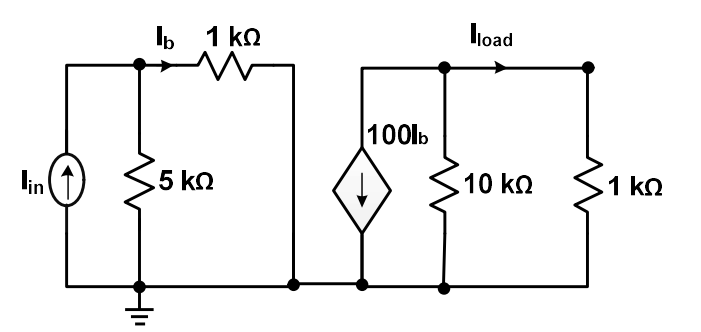
\includegraphics[width=0.6\columnwidth]{figs/q52.png}
\end{figure}

\qfooter

% Q.53
\item The linear temperature coefficient of the material of a wire is \(x \times 10^{-3} \,^\circ C^{-1}\).
The resistance of this wire increased from 50 \(\Omega\) at 25\(^\circ\)C to 60 \(\Omega\) at 75\(^\circ\)C.
The value of \(x\) is \rule{2cm}{0.15mm} (rounded off to two decimal places).

\qfooter

% Q.54
\item A series RLC circuit is connected to 220 V, 50 Hz supply. For a fixed value of R and C, the inductor L is varied to deliver the maximum current.
This value is 0.4 A and the corresponding potential drop across the capacitor is 330 V.
The value of the inductor L is \rule{2cm}{0.15mm} H (rounded off to two decimal places).

\qfooter

% Q.55
\item In the circuit diagram shown below, the MOSFET is biased in saturation region.
The MOSFET has threshold voltage \(V_{th} = 0.5\,V\), width \(W=100\,\mu m\), length \(L=0.1\,\mu m\), and \(\mu C_{ox} = 100\,\mu A/V^2\).
Assuming \(v_{in} = 1\,mV\) as a small-signal input to MOSFET, the magnitude of the output voltage \(V_{out}\) is \rule{2cm}{0.15mm} mV (accurate to two decimal places).
Ignore channel-length modulation.

\begin{figure}[H]
    \centering
    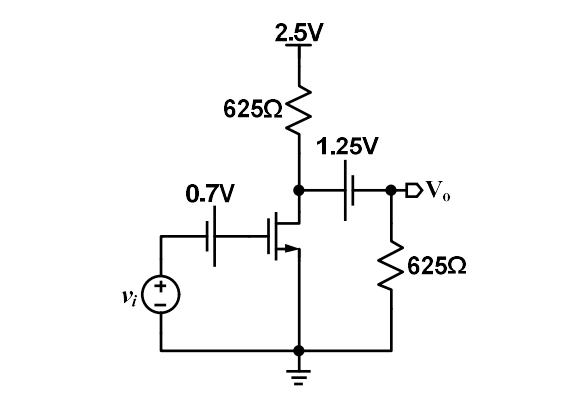
\includegraphics[width=0.6\columnwidth]{figs/q55.png}
\end{figure}

\qfooter

% Q.56
\item In the circuit diagram shown below, BJTs are biased with \(V_{BE} = 0.7\,V\).
Neglect the base current for operating point calculations.
Assume infinite input and output impedance for the BJTs.
The output voltage \(V_{out}\) with small input voltage \(v_{in} = 10\,mV\) is \rule{2cm}{0.15mm} mV (rounded off to one decimal place).
The thermal voltage \(V_T = 25\,mV\) at room temperature.

\begin{figure}[H]
    \centering
    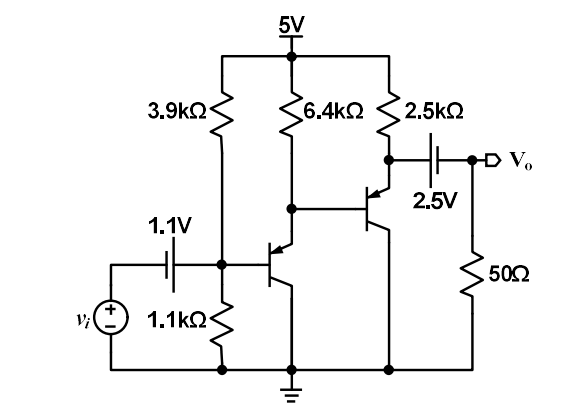
\includegraphics[width=0.6\columnwidth]{figs/q56.png}
\end{figure}

\qfooter

% Q.57
\item An ideal opamp with infinite gain and infinite bandwidth is connected in feedback as shown below.
The output voltage \(V_{out}\) for the given input voltages is \rule{2cm}{0.15mm} V (accurate to one decimal place).

\begin{figure}[H]
    \centering
    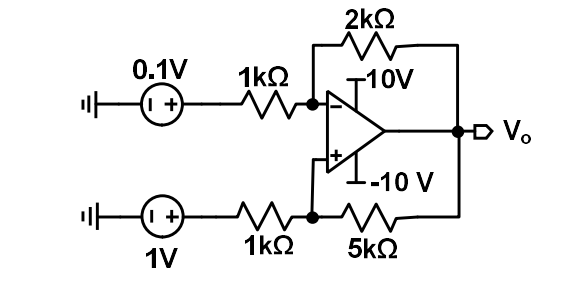
\includegraphics[width=0.6\columnwidth]{figs/q57.png}
\end{figure}

\qfooter

% Q.58
\item Independent voltage measurements \((\mu \pm \sigma)\) of three sensors where \(\mu\) and \(\sigma\) are mean and standard deviation respectively are:
\(v_1 = 4.52 \pm 0.02\,V\),
\(v_2 = 4.21 \pm 0.20\,V\),
\(v_3 = 3.96 \pm 0.15\,V\).
The measurement uncertainty in \(v_1 + v_2 + v_3\) is \rule{2cm}{0.15mm} V (rounded off to two decimal places).

\qfooter

% Q.59
\item A moving coil voltmeter has an internal resistance of 50 \(\Omega\).
The scale of the meter is divided into 100 equal divisions.
When a potential of 1 V is applied to terminals of voltmeter, a deflection of 100 divisions is obtained.
However, it is desired that when a potential of 500 V is applied to the terminals, a deflection of 100 divisions should be obtained.
The value of resistance that needs to be connected in series to achieve this is \rule{2cm}{0.15mm} \(\Omega\).

\qfooter

% Q.60
\item A Hall effect flow meter is used to measure the volumetric flow through a blood vessel.
The flow meter induces a magnetic field across the vessel and uses a voltmeter to measure voltage across the vessel, which is normal to both magnetic field and blood flow.
A caliper is used to measure the vessel diameter.
The system calculated flow rate as 100 cm\(^3\)/s using known magnetic field and measured voltage and diameter values.
After calibration, it was discovered the voltmeter was measuring 40% larger than actual and the caliper was measuring diameter 10% smaller than actual.
Assuming uniform flow profile and ignoring viscosity, the actual blood flow is \rule{2cm}{0.15mm} cm\(^3\)/s (rounded off to two decimal places).

\qfooter

% Q.61
\item A catheter-based arterial blood pressure measurement device uses a flexible diaphragm mounted with four identical strain gauges in a Wheatstone bridge configuration as shown in the figure.
Strain gauges have nominal resistance \(R_G = 10\,k\Omega\), Gauge Factor \(G = 40\), Young’s Modulus \(E = 10\,MPa\).
Blood pressure variations result in small finite positive strain \(\epsilon\).
If \(V_o\) is output voltage of Wheatstone bridge and \(\sigma\) is stress in MPa, the sensitivity \(\frac{V_o}{\sigma}\) is \rule{2cm}{0.15mm} V.MPa\(^{-1}\).

\begin{figure}[H]
    \centering
    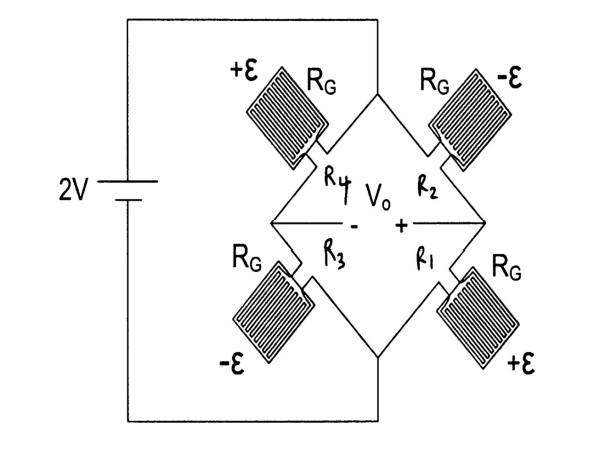
\includegraphics[width=0.6\columnwidth]{figs/q61.png}
\end{figure}

\qfooter

% Q.62
\item A patient has a breathing rate of 18 breaths per minute, tidal volume 500 mL, and anatomical dead space 150 mL.
If the person has a heart rate of 120 beats per minute and stroke volume of 50 mL, the alveolar ventilation to perfusion ratio is \rule{2cm}{0.15mm} (accurate to two decimal places).

\qfooter

% Q.63
\item Assume ratio of total blood volume in liters to total body weight in kg is 0.07.
The blood consists of plasma and RBCs only.
The plasma volume of a 70-kg man with 52% hematocrit is \rule{2cm}{0.15mm} L (rounded off to two decimal places).

\qfooter

% Q.64
\item The 1st generation (1G) CT scanner uses a point X-ray source and detector.
The source-detector assembly can move linearly at 0.5 m/s, and it takes 0.5 s for source-detector assembly to rotate one angular increment, regardless of angle.
This scanner is expected to collect 360 projections over 180° span.
The field of view diameter used for data collection is 0.5 m.
The scan time required is \rule{2cm}{0.15mm} s.

\qfooter

% Q.65
\item The inverse square law has a practical use in radiography.
While taking an acceptable chest radiograph of a subject 0.75 m from the X-ray generator, settings were 50 kVp, 50 mA.s.
If the subject is moved to 1 m and kVp is unchanged, the new value of mA.s to get the same exposure will be \rule{2cm}{0.15mm} mA.s (rounded off to two decimal places).

\qfooter

\end{enumerate}

\end{document}
